\documentclass[11pt]{article}
\usepackage[T1]{fontenc}
\usepackage[utf8]{inputenc}
\usepackage{amsmath, amssymb, amsfonts}
\usepackage{bm}
\usepackage{amsthm}
\usepackage{xcolor}
\usepackage{graphicx}
\usepackage{tikz}
\usetikzlibrary{arrows,positioning}
\usepackage{tcolorbox}
\tcbuselibrary{skins,breakable}

\newtheorem{theorem}{Theorem}
\definecolor{personalcontribcolor}{RGB}{30,136,229}
\definecolor{k3color}{RGB}{233,30,99}
\newcommand{\ReLU}{\mathrm{ReLU}}
\newcommand{\Kop}{\boldsymbol{\Theta}}

\begin{document}

\textbf{Multi-Component Multi-layer Neural Networks (MMNN)} and \textbf{Transformers}. 
The motivation for this focus stems from recent theoretical and empirical evidence demonstrating that these models can achieve
 remarkable \textbf{super-convergence} properties. This behavior suggests that their designs incorporate powerful implicit 
 preconditioning mechanisms that are not yet fully understood. Our goal is to dissect these architectures through the lens 
 of the NTK (NTK), a theoretical tool that connects an infinitely wide neural network to a linear model
  with a fixed kernel. By studying the spectral properties of the NTK for these models, we can gain deep insights into how
   their architectural choices influence the optimization dynamics and lead to such exceptional performance.



\subsection{Multi-Component Multi-layer Neural Networks (MMNN) and Transformers}

We examine Multi-Component Multi-layer Neural Networks (MMNN) and Transformer architectures, focusing on NTK preconditioning techniques. This means we investigate how to change our architectural
and training higher parameters (activation function, residual connections, message passing). At the time this report is written, most of the research is currently in progress.

For MMNN architectures, the kernel structure exhibits exhibits more stability. The preconditioning strategy decomposes the weight matrix into trainable/frozen weights,
and make the loss landscape less dimensionnal, and hopefully more convex. We present all the mathematical results and proofs
that are necessary to answer this question.

For Transformer models, the attention mechanism introduces non-linearities complicating kernel analysis. 
We introduce specialized techniques to handle softmax normalization within attention heads, in order to perform fast numerical experiments to compute
intractable quantities appearing. We provide also physical approximations strategies that will be used to perform the final step, and an agenda
to answer the question for this architecture.

\subsection{Feature Learning vs Kernel Regimes}

The transition between feature learning and kernel regimes represents a fundamental dichotomy in deep learning theory. In the kernel regime, network parameters remain close to initialization and the model behaves as a linear predictor in the NTK-defined feature space. Conversely, the feature learning regime allows significant parameter evolution, enabling adaptation of internal representations.

The NTK spectrum, particularly its smallest eigenvalue $\lambda_{\min}$, determines convergence rates and optimization strategy. An ill-conditioned NTK suggests second-order methods are appropriate, while a well-conditioned NTK indicates first-order methods can achieve faster convergence. For MMNN architectures, different network components may operate in different regimes simultaneously, requiring careful analysis of heterogeneous optimization dynamics.

\begin{tcolorbox}[colback=red!5,colframe=red!80!black,title={\textbf{Theorem: Spectral Equivalence of NTK, Hessian, and Fisher Matrix}},enhanced,drop shadow,boxrule=2pt]
A fundamental result in deep learning theory establishes that for sufficiently wide neural networks (width $m \to \infty$), the spectra of the Hessian, the Fisher Information Matrix, and the NTK (NTK) are asymptotically equivalent.

More precisely, the top $d$ eigenvalues of these matrices, where $d$ is the input data dimension, are proven to converge to the same limiting values determined by the NTK. The remainder of the spectrum, the "bulk," is concentrated around zero. It is provably shown that the spectral radius of this bulk decays as $\mathcal{O}(1/\sqrt{m})$. Furthermore, experimental results in []~\ref{takeuchi2025neuraltangentkernelsfisher} and []~\ref{dyer2019asymptotics} indicate that the individual non-top eigenvalues decay even faster, scaling as $\mathcal{O}(1/m)$. This powerful result connects the geometry of the loss landscape (Hessian) and information geometry (Fisher) to the kernel function, providing a unified view on optimization dynamics.
\end{tcolorbox}


\begin{tcolorbox}[colback=green!15,colframe=green!80!black,title={\textbf{Conjecture from Pr Haizhao Yang: Global Minima Stability}},enhanced,drop shadow,boxrule=2pt]
For sufficiently wide MMNN and Transformer networks, global minima exhibit a high local stability property ensuring convergence from neighborhoods around optimal solutions. The Hessian and NTK eigenvalues near global minima satisfy regularity conditions guaranteeing stable optimization dynamics.
\end{tcolorbox}


This conjecture is supported by numerical experiments []~\ref{zhang2024superconvergence} demonstrating super-convergence behavior in practical training scenarios.
By means of local analysis. Our goal now is to develop all the theoretical framework to have the tool to prove this conjecture. 
What we should prove is that the NTK is not moving too much near a global optima. We made a huge path towards this goal and are currently
holding stealth proofs for more general and smallest eigenvalue bounds that will be revealed in future works.


\newpage

\section{MMNN Model Definition and Asymptotic Regime}

\begin{tcolorbox}[colback=green!15,colframe=green!80!black,title={\textbf{Objective and Scope}},enhanced,drop shadow,boxrule=2pt]
This work derives the NTK $\boldsymbol{\Theta}$ operator of a Multi-layer Mean-field Matrix-Normal Network \textbf{(MMNN)}. 
The kernel is computed with respect to a specific set of trainable parameters, under the standard \textbf{"NTK parameterization"} 
which ensures a well-defined infinite-width limit.
\end{tcolorbox}


\begin{figure}[htbp]
    \centering
    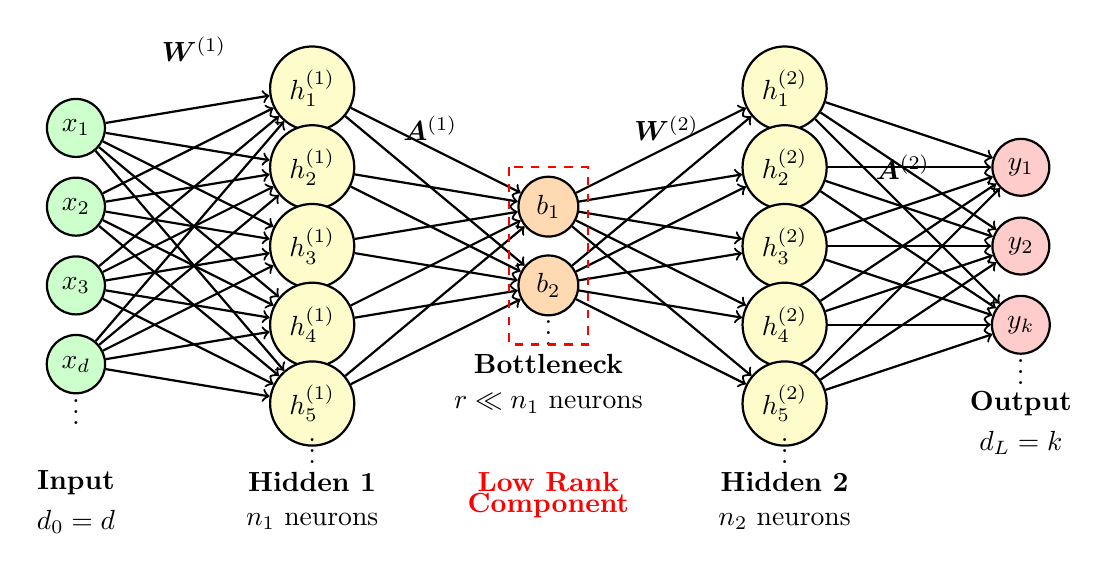
\begin{tikzpicture}[
        node distance=2cm and 3cm,
        neuron/.style={circle, draw, fill=blue!20, minimum size=15pt},
        input/.style={circle, draw, fill=green!20, minimum size=15pt},
        output/.style={circle, draw, fill=red!20, minimum size=15pt},
        hidden/.style={circle, draw, fill=yellow!20, minimum size=15pt},
        bottleneck/.style={circle, draw, fill=orange!30, minimum size=15pt},
        thick
    ]
    
    % Input layer
    \node[input] (x1) at (0,2) {$x_1$};
    \node[input] (x2) at (0,1) {$x_2$};
    \node[input] (x3) at (0,0) {$x_3$};
    \node[input] (xd) at (0,-1) {$x_d$};
    \node at (0,-1.5) {$\vdots$};
    
    % First hidden layer
    \node[hidden] (h11) at (3,2.5) {$h_1^{(1)}$};
    \node[hidden] (h12) at (3,1.5) {$h_2^{(1)}$};
    \node[hidden] (h13) at (3,0.5) {$h_3^{(1)}$};
    \node[hidden] (h14) at (3,-0.5) {$h_4^{(1)}$};
    \node[hidden] (h15) at (3,-1.5) {$h_5^{(1)}$};
    \node at (3,-2) {$\vdots$};
    
    % Bottleneck layer (low rank)
    \node[bottleneck] (b1) at (6,1) {$b_1$};
    \node[bottleneck] (b2) at (6,0) {$b_2$};
    \node at (6,-0.5) {$\vdots$};
    
    % Second hidden layer
    \node[hidden] (h21) at (9,2.5) {$h_1^{(2)}$};
    \node[hidden] (h22) at (9,1.5) {$h_2^{(2)}$};
    \node[hidden] (h23) at (9,0.5) {$h_3^{(2)}$};
    \node[hidden] (h24) at (9,-0.5) {$h_4^{(2)}$};
    \node[hidden] (h25) at (9,-1.5) {$h_5^{(2)}$};
    \node at (9,-2) {$\vdots$};
    
    % Output layer
    \node[output] (y1) at (12,1.5) {$y_1$};
    \node[output] (y2) at (12,0.5) {$y_2$};
    \node[output] (yk) at (12,-0.5) {$y_k$};
    \node at (12,-1) {$\vdots$};
    
    % Connections input to first hidden
    \foreach \i in {1,2,3,d} {
        \foreach \j in {11,12,13,14,15} {
            \draw[->] (x\i) -- (h\j);
        }
    }
    
    % Connections first hidden to bottleneck
    \foreach \i in {11,12,13,14,15} {
        \foreach \j in {1,2} {
            \draw[->] (h\i) -- (b\j);
        }
    }
    
    % Connections bottleneck to second hidden
    \foreach \i in {1,2} {
        \foreach \j in {21,22,23,24,25} {
            \draw[->] (b\i) -- (h\j);
        }
    }
    
    % Connections second hidden to output
    \foreach \i in {21,22,23,24,25} {
        \foreach \j in {1,2,k} {
            \draw[->] (h\i) -- (y\j);
        }
    }
    
    % Layer labels
    \node at (0,-2.5) {\textbf{Input}};
    \node at (0,-3) {$d_0 = d$};
    
    \node at (3,-2.5) {\textbf{Hidden 1}};
    \node at (3,-3) {$n_1$ neurons};
    
    \node at (6,-1) {\textbf{Bottleneck}};
    \node at (6,-1.5) {$r \ll n_1$ neurons};
    
    \node at (9,-2.5) {\textbf{Hidden 2}};
    \node at (9,-3) {$n_2$ neurons};
    
    \node at (12,-1.5) {\textbf{Output}};
    \node at (12,-2) {$d_L = k$};
    
    % Mathematical notation
    \node at (1.5,3) {$\bm{W}^{(1)}$};
    \node at (4.5,2) {$\bm{A}^{(1)}$};
    \node at (7.5,2) {$\bm{W}^{(2)}$};
    \node at (10.5,1.5) {$\bm{A}^{(2)}$};
    
    % Highlight low rank structure
    \draw[red, thick, dashed] (5.5,1.5) rectangle (6.5,-0.75);
    \node[red] at (6,-2.5) {\textbf{Low Rank}};
    \node[red] at (6,-2.8) {\textbf{Component}};
    
    \end{tikzpicture}
    \caption{Architecture of a Multi-component Multi-layer Neural Network (MMNN) with a low-rank intermediate layer. The red dashed connections indicate the low-rank component that reduces dimensionality from $n_1$ to $r \ll n_1$ neurons.
    We only train the output weights $\bm{A}^{(1)}$ and $\bm{A}^{(2)}$.}
    \label{fig:mmnn_architecture}
\end{figure}


\subsection{Personal contribution : NTK initialization for MMNN Architecture}

\begin{tcolorbox}[colback=yellow!15,colframe=yellow!80!black,title={\textbf{Definition: MMNN Architecture}},enhanced,drop shadow,boxrule=2pt]
We consider an \textbf{MMNN} of depth $L$. Let the input be $\bm{h}^{(0)}(\bm{x}) = \bm{x} \in \mathbb{R}^{d_0}$. For each layer $\ell = 1, \dots, L$, the output $\bm{h}^{(\ell)}$ is defined recursively:

\begin{equation}
    \bm{h}^{(\ell)}(\bm{x}) = \frac{\sigma_A}{\sqrt{n_\ell}} \sum_{j=1}^{n_\ell} \bm{A}_j^{(\ell)} \ReLU\left(\bm{w}_j^{(\ell)\top} \bm{h}^{(\ell-1)}(\bm{x}) + \beta b_j^{(\ell)}\right) + \sigma_c \bm{c}^{(\ell)}
\end{equation}

where $n_\ell$ is the width of layer $\ell$ and $\bm{h}^{(\ell)} \in \mathbb{R}^{d_\ell}$.
\end{tcolorbox}



\begin{tcolorbox}[colback=blue!15,colframe=blue!80!black,title={\textbf{Remark : Parameter Classification}},enhanced,drop shadow,boxrule=2pt]
The parameters for each layer are divided into two groups:

\textbf{1. Trainable Parameters:} The output weights $\{\bm{A}_j^{(\ell)}\}_{j=1}^{n_\ell}$ and biases $\bm{c}^{(\ell)}$ are optimized during training. The NTK $\Kop $ is computed with respect to these parameters.

\textbf{Initialization:}
\begin{itemize}
\item The weights $\bm{A}_j^{(\ell)} \sim \mathcal{N}(0, 1)$. The term $\frac{\sigma_A}{\sqrt{n_\ell}}$ is the \textbf{NTK parameterization}, ensuring kernel convergence as $n_\ell \to \infty$.
\item The bias $\bm{c}^{(\ell)} \sim \mathcal{N}(0, 1)$ is initialized at zero with scaling $\sigma_c$.
\end{itemize}

\textbf{2. Random Parameters:} The input weights $\bm{w}_j^{(\ell)}$ and biases $b_j^{(\ell)}$ are randomly initialized and \textbf{fixed} throughout training.
\end{tcolorbox}



\begin{tcolorbox}[colback=green!5,colframe=green!80!black,title={\textbf{Insight : Architectural Philosophy}},enhanced,drop shadow,boxrule=2pt]
This random basis initialization is chosen on purpose, supported by approximation theorems []~\ref{zhang2024superconvergence}, with intuition from localizing high frequency variations.
With this method, we reduce the number of parameters from $n_\ell^2$ to $n_\ell * d_\ell$.

The NTK parameterization is chosen to ensure a well-defined infinite-width limit. The $\mu$ parameterization do not have this property.
\end{tcolorbox}



\subsection{Personal contribution : Parameterization and Training Regime}

The choice of parameterization fundamentally determines the network's behavior in the infinite-width limit. We distinguish two main regimes that correspond to distinct learning philosophies. The first, NTK parameterization, favors stability and convergence toward a linear model, while the second, mean-field parameterization, promotes feature learning and non-linear dynamics.

\begin{tcolorbox}[colback=green!5,colframe=green!80!black,title={\textbf{Remark: Critical Parameterization Choice}},enhanced,drop shadow,boxrule=2pt]
The choice of scaling for the trainable parameters critically determines the network's behavior in the infinite-width limit. 

\textbf{1. NTK Parameterization (Our approach):} We use the $\frac{1}{\sqrt{n_\ell}}$ scaling for output weights.
\begin{itemize}
\item Output function $h^{(\ell)}(x)$ maintains variance $\mathcal{O}(\sigma_A^2)$ → \textbf{stable magnitude preservation}
\item Gradient with respect to weights remains small: $\mathcal{O}(\frac{1}{\sqrt{n_\ell}})$ → \textbf{"lazy training" regime}
\item Network dynamics converge to linear model behavior characterized by the NTK
\end{itemize}

\textbf{2. Mean-Field ($\mu$) Parameterization []~\ref{yang2020meanfield}:} Alternative $\frac{1}{n_\ell}$ scaling.
In this parameterization, function outputs are of order $\mathcal{O}(\frac{1}{\sqrt{n_\ell}})$ while gradients remain of order $\mathcal{O}(1)$, enabling unit-scale parameter updates. This scaling is termed "mean-field" because each neuron's contribution is of order $\mathcal{O}(1)$, allowing collective influence of all neurons. This configuration promotes feature learning and non-linear dynamics.

Those initialization are opposite, and we will see that the NTK parameterization is the best for the MMNN architecture to have order one gaussianity in low rank layers.
\end{tcolorbox}






\begin{tcolorbox}[colback=yellow!5,colframe=yellow!80!black,title={\textbf{Definition: Neural Network Gaussian Process (NNGP)}},enhanced,drop shadow,boxrule=2pt]
For a given layer $\ell$, when $n_\ell \to \infty$, the output $\bm{h}^{(\ell)}(\bm{x})$ converges in 
distribution to a composition of Gaussian processes whose covariance conditioned to the previous layer is determined by the NNGP kernel $\mathcal{K}_{NNGP}^{(\ell | \ell-1)}$.

We have:
\begin{equation}
\mathcal{K}_{NNGP}^{(\ell | \ell-1 )}(\bm{x}, \bm{x}') = \text{Cov}\left[\bm{h}^{(\ell)}(\bm{x}), \bm{h}^{(\ell)}(\bm{x}') \mid \bm{h}^{(\ell-1)}\right]
\end{equation}
\end{tcolorbox}

\begin{tcolorbox}[colback=red!10,colframe=red!80!black,title={\textbf{Crucial Remark: Composition of Gaussian Processes}},enhanced,drop shadow,boxrule=2pt]
\textbf{Fundamental point:} In this limit, the output of each layer $\bm{h}^{(\ell)}$ converges in distribution to a \textbf{composition of Gaussian Processes (GP)} which is \textbf{not} itself a Gaussian process!

Consequently, the NNGP and NTK kernels for layers $\ell > 1$, which are functions of the output of the previous layer, 
remain \textbf{random quantities} (random fields). This is different from FCNNs but we use the same terminology on purpose.
The recursive formulas describe the relationship between these random kernels.

This distinction is crucial because:
\begin{itemize}
\item For $\ell = 1$: $\bm{h}^{(1)}$ is Gaussian → $\mathcal{K}_{NNGP}^{(1)}$ and $\Theta^{(1)}$ are deterministic
\item For $\ell > 1$: $\bm{h}^{(\ell)}$ is composition of GP → $\mathcal{K}_{NNGP}^{(\ell)}$ and $\Theta^{(\ell)}$ are random
\end{itemize}

The recursion captures the evolution of these kernel distributions through the layers.
\end{tcolorbox}




\subsection{Personal contribution : Asymptotic Regime}
The entire NTK and NNGP formalism relies on the infinite-width limit giving gaussianity. Following the framework established by []~\ref{jacot2018ntk}, we analyze the network in a specific asymptotic regime:
\begin{itemize}
    \item The dimensions of the hidden layers, or widths, $n_1, n_2, \dots, n_L$ are taken to infinity.
    \item The input and output dimensions of each layer ($d_0, d_1, \dots, d_L$) are kept fixed and finite.
    \item Critically, the limits are taken sequentially: first we let $n_1 \to \infty$, then $n_2 \to \infty$, and so on up to $n_L \to \infty$.
    \item 
\end{itemize}
\begin{tcolorbox}[colback=green!5,colframe=green!80!black,title={\textbf{Remark: Sequential Limit as Key Theoretical Tool}},enhanced,drop shadow,boxrule=2pt]
This sequential limit is the key theoretical tool. When analyzing layer $\ell$ in the limit $n_\ell \to \infty$, the output of the previous layer, $\bm{h}^{(\ell-1)}$, is a sum of an infinite number of i.i.d. random variables (by construction of layer $\ell-1$). By the Central Limit Theorem, $\bm{h}^{(\ell-1)}$ converges in distribution to a Gaussian Process. This allows us to replace the complex, random function $\bm{h}^{(\ell-1)}$ with a GP whose covariance structure is precisely the NNGP kernel $\Sigma^{(\ell-1)}$. This is the foundation of the recursive calculation.
\end{tcolorbox}

\subsection{Personal contribution : Signal Propagation and the Edge of Chaos (EOC)}
Before analyzing the kernel, we study the propagation of the signal's magnitude through the network at initialization. We are interested in the evolution of the variance of the layer outputs, defined as $q^{(\ell)} = \mathbb{E}[\|\bm{h}^{(\ell)}\|^2]/d_\ell$.

For a ReLU activation and assuming centered parameters, the variance evolves according to the following recurrence relation (see Appendix for proof):
\begin{equation}
    q^{(\ell)} = \sigma_c^2 + \frac{\sigma_A^2}{2} \left( q^{(\ell-1)}\text{Tr}(\Sigma_w) + \beta^2 \right)
\end{equation}
This is an affine map $q^{(\ell)} = M \cdot q^{(\ell-1)} + C$. For the signal to propagate stably without vanishing ($M<1$) or exploding ($M>1$), the dynamics must be at the "Edge of Chaos", where the factor is exactly 1.

% \begin{block}
\begin{tcolorbox}[colback=red!15,colframe=red!80!black,title={\textbf{Edge of Chaos Condition}},enhanced,drop shadow,boxrule=2pt]

The condition for stable signal propagation is:
\begin{equation}
    \frac{\sigma_A^2}{2} \text{Tr}(\Sigma_w) = 1 \quad \implies \quad \sigma_A \sqrt{\text{Tr}(\Sigma_w)} = \sqrt{2}
\end{equation}
We call the EOC initialization when adding the condition $\sigma_c^2 =1$.
\end{tcolorbox}
% \end{block}


\begin{theorem}[Gaussian process]

For a layer $\ell$ with output dimension $d_\ell$, the layer output $\bm{h}^{(\ell)}(\bm{x})$ follows a $d_\ell$-dimensional Gaussian process with Kronecker covariance structure:

\begin{equation}
\boxed{\bm{h}^{(\ell)} \sim \mathcal{GP}(0, \mathbf{M}^{(\ell)} \otimes \mathbf{I}_{d_\ell})}
\end{equation}

where $\mathbf{M}^{(\ell)}$ is the 2-dimensional covariance matrix between different input points:
\begin{equation}
\mathbf{M}^{(\ell)}_{i,j} = \text{Cov}(h^{(\ell)}_k(\bm{x}_i), h^{(\ell)}_k(\bm{x}_j)) = \sigma_c^2 + \rho^{(\ell)}(\bm{x}_i, \bm{x}_j)
\end{equation}

and $\mathbf{I}_{d_\ell}$ is the $d_\ell \times d_\ell$ identity matrix clek!rnapturing the independence across output dimensions within the same input point.

\end{theorem}




\newpage

\section{NTK formulas for MMNNs}

\subsection{Personal contribution : NTK for a Single-Layer MMNN}
\label{sec:single_layer_mmfn}
We begin by deriving the NTK for a single-layer MMNN. This result forms the base case for the multi-layer recursion. For simplicity, we consider a single scalar output, such that the network is defined as:

\begin{tcolorbox}[colback=yellow!10,colframe=yellow!80!black,title={\textbf{Single-Layer MMNN Definition}},enhanced,drop shadow,boxrule=2pt]
\begin{equation}
    \boxed{h(\bm{x}) = \frac{1}{\sqrt{n}} \sum_{j=1}^n A_j \ReLU(\bm{w}_j^\top \bm{x} + b_j) + c}
\end{equation}
The trainable parameters are $\theta = \{A_j\}_{j=1}^n \cup \{c\}$. The parameters $\{\bm{w}_j, b_j\}$ are fixed and randomly drawn, with $\bm{w}_j \sim \mathcal{N}(0, \Sigma_w)$ and $b_j \sim \mathcal{N}(\mu_b, \sigma_b^2)$.
\end{tcolorbox}

\subsection{From Gradient Products to an Expectation}
In the infinite-width limit ($n \to \infty$), the NTK converges to a rotation invariant kernel (hence zonal) as an expectation over the distribution of the random parameters $(\bm{w}, b)$. The full NTK is the sum of the kernel part from the weights $\{A_j\}$ and the part from the bias $\{c\}$.

\begin{tcolorbox}[colback=blue!10,colframe=blue!80!black,title={\textbf{NTK as Expectation}},enhanced,drop shadow,boxrule=2pt]
\begin{equation}
\label{eq:ntk_expectation}
    \boxed{\Theta^{(1)}(\bm{x}, \bm{x}') = \underbrace{\mathbb{E}_{\bm{w},b} \left[ \ReLU(\bm{w}^\top \bm{x} + b)\ReLU(\bm{w}^\top \bm{x}' + b) \right]}_{\text{NNGP Kernel } \Sigma^{(1)}(\bm{x}, \bm{x}')} + \underbrace{\sigma_c^2}_{\text{from bias } c}}
\end{equation}
\end{tcolorbox}

\subsection{Personal contribution : Integral Formulation and Parameter Mapping}
The NNGP kernel $\Sigma^{(1)}$ is an integral over the distributions of $\bm{w}$ and $b$:
\begin{equation}
    \Sigma^{(1)}(\bm{x}, \bm{x}') = \int_{\mathbb{R}^d} \int_{\mathbb{R}} \ReLU(\bm{w}^\top \bm{x} + b)\ReLU(\bm{w}^\top \bm{x}' + b) p(\bm{w})p(b) \,db \,d\bm{w}
\end{equation}

A change of variables is performed from the parameter space $(\bm{w}, b)$ to the pre-activation space $(g_1, g_2)$, where $g_1 = \bm{w}^\top \bm{x} + b$ and $g_2 = \bm{w}^\top \bm{x}' + b$. This transforms the high-dimensional integral into an expectation over a 2D bivariate Gaussian distribution. The parameters of this distribution are:

\begin{tcolorbox}[colback=green!5,colframe=green!80!black,title={\textbf{Remark: Bivariate Gaussian Parameters}},enhanced,drop shadow,boxrule=2pt]
\begin{itemize}
    \item \textbf{Means:} $\mu_1 = \mathbb{E}[g_1] = \mathbb{E}[\bm{w}^\top\bm{x} + b] = \mu_b$. By symmetry, $\mu_2 = \mu_b$.
    \item \textbf{Variances:} $\sigma_1^2 = \text{Var}(g_1) = \text{Var}(\bm{w}^\top\bm{x}) + \text{Var}(b) = \bm{x}^\top \Sigma_w \bm{x} + \sigma_b^2$. Similarly, $\sigma_2^2 = {\bm{x}'}^\top \Sigma_w \bm{x}' + \sigma_b^2$.
    \item \textbf{Covariance:} $\text{Cov}(g_1, g_2) = \mathbb{E}[(\bm{w}^\top\bm{x})(\bm{w}^\top\bm{x}')] + \text{Var}(b) = \bm{x}^\top \Sigma_w \bm{x}' + \sigma_b^2$.
\end{itemize}
\end{tcolorbox}

\subsection{Personal contribution : Final Analytical Expression}
\begin{theorem}[NNGP Kernel for a Single-Layer ReLU MMNN]
Let the pre-activations $(g_1, g_2)$ be jointly Gaussian with parameters $(\mu_1, \sigma_1^2)$ and $(\mu_2, \sigma_2^2)$ and correlation $\rho$. The NNGP kernel $\Sigma^{(1)} = \mathbb{E}[\text{ReLU}(g_1)\text{ReLU}(g_2)]$ is given by the decomposition:

\begin{tcolorbox}[colback=blue!10,colframe=blue!80!black,title={\textbf{NNGP Kernel Decomposition}},enhanced,drop shadow,boxrule=2pt]
\begin{equation}
\label{eq:final_ntk_decomp}
\boxed{
\Sigma^{(1)} = \sigma_1\sigma_2 \cdot I_{12} + \mu_1\sigma_2 \cdot I_{01} + \mu_2\sigma_1 \cdot I_{10} + \mu_1\mu_2 \cdot I_{00}
}
\end{equation}
where the terms $I_{ij}$ are moments of standardized bivariate normal variables $(Z_1, Z_2)$ with thresholds $a_1 = -\mu_1/\sigma_1$ and $a_2 = -\mu_2/\sigma_2$.
\end{tcolorbox}
\end{theorem}












\end{document}




\subsection{Personal contribution : Recursion for Multi-Layer MMNNs}
We now extend the single-layer result to deep networks. The recursion involves two distinct but intertwined random fields: the NNGP kernel $\Sigma^{(\ell)}$ and the NTK kernel $\Theta^{(\ell)}$.

\begin{tcolorbox}[colback=red!10,colframe=red!80!black,title={\textbf{Crucial Remark: Random Kernels in Deep Networks}},enhanced,drop shadow,boxrule=2pt]
An important fact is that the NNGP kernel $\Sigma^{(\ell)}$ is a random field that is NOT a gaussian process but a deep gaussian process, while the NTK kernel $\Theta^{(\ell)}$ is also a random field that is not a gaussian process. This is because the composition of a non-linear function with a Gaussian Process, $g(f(x))$, is not, in general, a Gaussian Process.
\end{tcolorbox}

\subsection{NNGP Kernel \(\Sigma^{(\ell)}\) Recursion}
The NNGP kernel describes the covariance of the network's output function at initialization. For any finite width, this output is a random function. In the infinite-width limit, it converges to a Gaussian Process. The base kernel $\Sigma^{(\ell)}$ is defined recursively.

\begin{tcolorbox}[colback=blue!10,colframe=blue!80!black,title={\textbf{NNGP Kernel Recursion}},enhanced,drop shadow,boxrule=2pt]
\begin{itemize}
    \item \textbf{Base Case (\(\ell=1\)):} The NNGP kernel for the first layer:
    \begin{equation}
        \boxed{\Sigma^{(1)}(x, x') = \mathbb{E}_{\bm{w},b}\left[\ReLU(\bm{w}^\top x + b)\ReLU(\bm{w}^\top x' + b)\right]}
    \end{equation}
    \item \textbf{Recursive Step (\(\ell > 1\)):} For subsequent layers:
    \begin{equation}
        \boxed{\Sigma^{(\ell)}(x, x') = \mathbb{E}_{\bm{w}, b} \left[ \ReLU\left(\bm{w}^\top \bm{h}^{(\ell-1)}(x) + \beta b\right) \ReLU\left(\bm{w}^\top \bm{h}^{(\ell-1)}(x') + \beta b\right) \right]}
    \end{equation}
\end{itemize}
\end{tcolorbox}















\subsection{Personal contribution: NTK Kernel \(\Theta^{(\ell)}\) Recursion}
The NTK is the Gram matrix of function gradients. For any finite width, it is a random matrix. The following recursion describes the relationship between these random kernels in the infinite-width limit.

\begin{tcolorbox}[colback=blue!10,colframe=blue!80!black,title={\textbf{NTK Recursion Formula}},enhanced,drop shadow,boxrule=2pt]
\begin{itemize}
    \item \textbf{Initialization (\(\ell=0\)):} $\Theta^{(0)} = 0$.
    
    \item \textbf{Recursive Step (\(\ell \ge 1\)):} The NTK for layer $\ell$ combines the NTK from previous layers with the contributions from the trainable parameters $A^{(\ell)}$ and $c^{(\ell)}$:
    \begin{equation}
        \boxed{
        \Theta^{(\ell)}(x, x') = \Theta^{(\ell-1)}(x, x') \cdot \left(\sigma_A^2\dot{\Sigma}^{(\ell)}(x, x')\right) + \sigma_A^2 \Sigma^{(\ell)}(x, x') + 1
        }
    \end{equation}
    where $\sigma_c^2=1$ is the contribution from the trainable bias. $\Sigma^{(\ell)}$ is the base NNGP kernel defined above. $\dot{\Sigma}^{(\ell)}$ is the base derivative kernel:
    \begin{equation}
        \dot{\Sigma}^{(\ell)}(x, x') = \mathbb{E}_{\bm{w}, b} \left[ \dot{\ReLU}\left(\bm{w}^\top \bm{h}^{(\ell-1)}(x) + \beta b\right) \dot{\ReLU}\left(\bm{w}^\top \bm{h}^{(\ell-1)}(x') + \beta b\right) \bm{w}^\top\bm{w} \right]
    \end{equation}
    with $\dot{\ReLU}$  being the derivative of the activation function. Both $\Sigma^{(\ell)}$ and $\dot{\Sigma}^{(\ell)}$ are random kernels for $\ell > 1$.
\end{itemize}
This recursion relation do not depend on EOC initialization, and that is why we do not replace $\sigma_A^2$ by its EOC counterpart
\end{tcolorbox}


\subsection{Parameter Influence on NTK Preconditioning}

\begin{tcolorbox}[colback=green!5,colframe=green!80!black,title={\textbf{Remark: Activation and Bias Influence on NTK}},enhanced,drop shadow,boxrule=2pt]
The NTK behavior can be systematically controlled through two key parameters that serve as natural preconditioning mechanisms:

\textbf{1. Activation Function Choice:} The choice of activation function directly and its convexity affect both $\Sigma^{(\ell)}$ and $\dot{\Sigma}^{(\ell)}$ kernels. For ReLU, we obtain specific analytical forms that enable tractable computations, while alternative activations (sigmoid, tanh) modify the kernel's spectral properties and convergence behavior.

\textbf{2. Bias Parameter $\boldsymbol{\beta}$:} The bias scaling $\beta$ controls NTK preconditioning. Setting $\beta = 0$ yields centered pre-activations, while $\beta > 0$ improves training stability. This provides direct control over the kernel's spectral properties.
\end{tcolorbox}








\subsection{Personal contribution: Two Hidden Layer MMNN Architecture NTK analysis}
\begin{tcolorbox}[colback=green!15,colframe=green!80!black,title={\textbf{Objective: Comparative Analysis of MMNN vs Standard MLP}},enhanced,drop shadow,boxrule=2pt]
The purpose of this analysis is to expose what the NTK should be when compared in the minimal setup against standard multi-layer perceptron. We consider a configuration with 2 hidden layers, where the low-rank structure is incorporated for MMNNs to demonstrate the fundamental differences in kernel behavior between these architectures.
\end{tcolorbox}

The considered architecture is:
\begin{center}
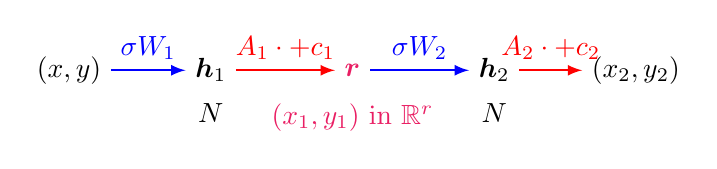
\begin{tikzpicture}[scale=0.6]
    \node (x) at (0,0) {$(x,y)$};
    \node (h1) at (3,0) {$\bm{h}_1$};
    \node (r) at (6,0) {$\textcolor{k3color}{\bm{r}}$};
    \node (h2) at (9,0) {$\bm{h}_2$};
    \node (y) at (12,0) {$(x_2,y_2)$};
    
    \draw[-latex,thick,blue] (x) -- node[above] {$\sigma W_1$} (h1);
    \draw[-latex,thick,red] (h1) -- node[above] {$A_1 \cdot+c_1$} (r);
    \draw[-latex,thick,blue] (r) -- node[above] {$\sigma W_2$} (h2);
    \draw[-latex,thick,red] (h2) -- node[above] {$A_2 \cdot +c_2$} (y);
    
    \node[below] at (3,-0.5) {$N$};
    \node[below] at (6,-0.5) {\textcolor{k3color}{$(x_1,y_1)$ in $\mathbb{R}^r$}};
    \node[below] at (9,-0.5) {$N$};
\end{tikzpicture}
\end{center}
\begin{tcolorbox}[colback=personalcontribcolor!10,colframe=personalcontribcolor,title={\textbf{Main Formula: Two Layer MMNN NTK}},enhanced,drop shadow]
For $\beta = 0$, the \textcolor{red}{\textbf{NTK}} for two hidden layers is written as:
\begin{align}
\textcolor{red}{\boldsymbol{\Theta}}^{(1)} &= \mathbb{E}_{\bm{w}} \left[ \sigma(\bm{w}^\top x) \sigma(\bm{w}^\top x') \right] + 1 \\
\textcolor{red}{\boldsymbol{\Theta}}^{(2)} &= \textcolor{red}{\boldsymbol{\Theta}}^{(1)} \cdot \left(\sigma_A^2 \mathbb{E}_{\bm{w}} \left[ \dot{\sigma}(\bm{w}^\top \bm{h}^{(1)}(x)) \dot{\sigma}(\bm{w}^\top \bm{h}^{(1)}(x')) \bm{w}^\top\bm{w} \right]\right) \nonumber\\
&\quad + \mathbb{E}_{\bm{w}} \left[ \sigma(\bm{w}^\top \bm{h}^{(1)}(x)) \sigma(\bm{w}^\top \bm{h}^{(1)}(x')) \right] + 1
\end{align}
\end{tcolorbox}





\begin{tcolorbox}[colback=green!15,colframe=green!80!black,title={\textbf{Ongoing Research: Deep Network Scaling via Lyapunov Analysis}},enhanced,drop shadow,boxrule=2pt]
The MMNN structure presented above is \textbf{particularly interesting} for analyzing deep networks with growing number of layers $L$. We can employ \textbf{Lyapunov analysis} to study the products of independent random variables that emerge through the layer-wise recursions. This approach allows us to derive the expected \textbf{scaling behavior with respect to depth $L$}, which is crucial for understanding the dynamics of very deep networks.

This scaling analysis through products of random matrices is precisely what we are pursuing in our \textbf{current investigations}, extending the two-layer results to arbitrary depth and characterizing the geometric properties of the resulting kernel evolution.
\end{tcolorbox}


\newpage
\subsection{Personal contribution : Final Result}

\begin{tcolorbox}[colback=personalcontribcolor!10,colframe=personalcontribcolor,title={\textbf{MAIN RESULT}},enhanced,drop shadow,breakable]
For 2 inputs $x,y \in \mathbb{S}^{d-1}$ with cosine similarity $\textcolor{magenta}{\rho}$ and a low-rank hidden layer $r$, the \textcolor{red}{\textbf{NTK}} for a two hidden layer EOC initialized MMNN is:

\begin{equation}
\boxed{\textcolor{red}{\boldsymbol{\Theta}}^{(2)}(x,y) = \boldsymbol{\tilde{\Theta}}^{(2)}(\textcolor{magenta}{\rho}) = \textcolor{red}{\boldsymbol{\Theta}}^{(1)}(\textcolor{magenta}{\rho_1}) \cdot \left(1 - \frac{\arccos(\textcolor{magenta}{\rho_1})}{\pi}\right)\frac{2}{r} + \frac{2}{r}\textcolor{red}{\boldsymbol{\Sigma}}^{(1)}(\textcolor{magenta}{\rho_1})\|x_1\| \|y_1\| + 1}
\end{equation}

with $\textcolor{red}{\boldsymbol{\Sigma}}^{(1)}(\textcolor{magenta}{\rho}) = \frac{1}{\pi}\left(\sqrt{1-\textcolor{magenta}{\rho}^2} + \textcolor{magenta}{\rho}(1-\arccos(\textcolor{magenta}{\rho}))\right)$

where the random variables follow:
\begin{itemize}
\item $\textcolor{magenta}{\rho_1} \sim \text{Fisher}(\textcolor{magenta}{\rho_1}, r)$ is independent of the norms ($\|x_1\|$, $\|y_1\|$)
\item $(\|x_1\|^2, \|y_1\|^2) \sim \text{Kibble}(r, \textcolor{magenta}{\rho_1})$ are chi-squared variables from correlated normal variables with $r$ degrees of freedom (scalar product is a sum of independent Bessel variables)
\end{itemize}
\end{tcolorbox} 
We explain more about those Fisher and Kibble distributions in appendix.


\begin{tcolorbox}[colback=green!10,colframe=green,title={\textbf{High-Dimensional Behavior}},enhanced]
For large values of $r$, Fisher's $z$-transformation gives $z = \text{arctanh}(\rho_1) \sim \mathcal{N}\left(\text{arctanh}(\rho) + \frac{\rho}{2(r-1)}, \frac{1}{r-3}\right)$. 

The variance of $\rho_1$ decreases as $O(1/r)$. When $\rho \sim O(1/\sqrt{r})$, geometric noise masks the correlation.

For the normalized product $S/r = \|\textcolor{red}{\mathbf{X}}\|\|\textcolor{red}{\mathbf{Y}}\|/r$, we have:
\begin{equation}
\boxed{\frac{S}{r} \xrightarrow{r \to \infty} 1}
\end{equation}
This convergence occurs with fluctuations of order $O(1/\sqrt{r})$.
\end{tcolorbox}

\begin{tcolorbox}[colback=green!10,colframe=green!80!black,title={\textbf{Remark: Fast Decay of NTK Fluctuations}},enhanced,drop shadow,boxrule=2pt]
The NTK fluctuations decay rapidly with rate $O(1/r)$, which implies that we obtain \textbf{trivial eigenvalue bounds} provided we can compute the deterministic zonal function $\boldsymbol{\tilde{\Theta}}(\rho)$. This fast convergence rate ensures that the random components of the kernel become negligible for moderate values of $r$, allowing us to approximate the spectral properties using the deterministic part of the kernel. The theoretical challenge thus reduces to analyzing the spectrum of the limiting zonal kernel operator.
Ongoing research is doing a taylor expansion of the NTK near $\rho =1$ on that purpose.
\end{tcolorbox}

\begin{tcolorbox}[colback=green!10,colframe=green!80!black,title={\textbf{Computational Insight: Linear Programming Formulation}},enhanced,drop shadow,boxrule=2pt]
Following []~\ref{zhang2024superconvergence} approach, uniform distributions for random weights $\bm{w}_j^{(\ell)} \sim \text{Uniform}(\mathcal{S}^{d_{\ell-1}})$ and biases $b_j^{(\ell)} \sim \text{Uniform}[-1,1]$ transform MMNN theoretical optimization into a \textbf{linear programming problem}.

Since the random basis functions $\sigma(\bm{w}_j^{(\ell)\top} \bm{h}^{(\ell-1)}(\bm{x}) + \beta b_j^{(\ell)})$ are fixed and the network output is linear in trainable weights $\{\bm{A}_j^{(\ell)}\}$, the optimization becomes convex and exactly solvable.
Another way to precondition the NTK is to choose a specific ad-hoc great initialization that we are trying to find in ongoing research.
\end{tcolorbox}











